\documentclass[english]{article}

%% Packages pull in extra commands:
%% http://en.wikibooks.org/wiki/LaTeX/Packages

\usepackage{hyperref}
\usepackage[latin9]{inputenc}
\usepackage[letterpaper]{geometry}
\geometry{verbose,tmargin=1in,bmargin=1in,lmargin=1in,rmargin=1in}
\usepackage{amsmath}
\usepackage{amssymb}
\usepackage{graphicx}
\usepackage{float}
\usepackage{array}
\usepackage{enumerate}
\usepackage{tikz}
\usepackage{bm}

% New commands serve as shorthand for frequently used command combinations.
\newcommand{\ind}[1]{\mathbf{1}\left(#1\right)}
\newcommand{\bx}{\mathbf{x}}
\newcommand{\E}{\mathbf{E}}

\title{CIS 520, Machine Learning, Fall 2018: Assignment 6}
\author{Shubhankar Patankar}

\begin{document}
\maketitle

% {\normalsize \noindent Collaborators: \\ 
% \\ \underline{ Type Collaborator Name Here        }} \\
\newpage

\section{CCA}
\begin{enumerate}
    \item CCA Projection Directions
    \begin{figure}[H]
    \centering
    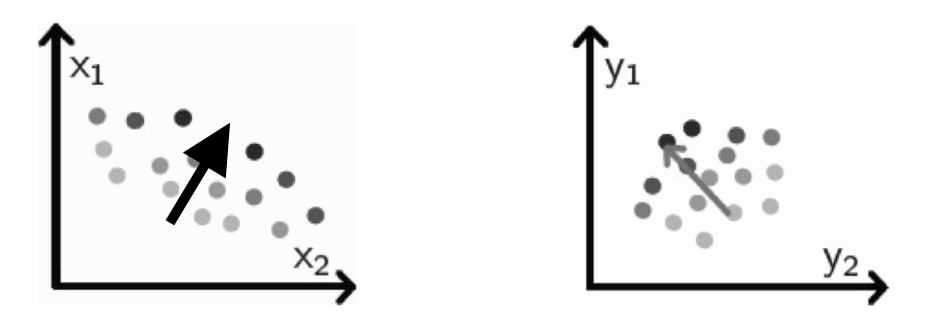
\includegraphics[scale = 0.5]{1_a}
    \caption{Projection Directions}
    \label{fig:1_a}
    \end{figure}
    \item Correlations
        \begin{enumerate}
        \item Correlation between $XU$ and $YV^T$ (CCA): $R = 0.9134$
        \item Correlation between $\hat{y}$ and $y$ using one PC: $R = 0.9098$. The result obtained from CCA is better correlated than the PCR version with one principal component.  
    \end{enumerate}
    	\textbf{Code for Problem 1}
	\color{black}
    	\begin{verbatim}
	clc; close all; clear;

%% 2 (a)

load('breast_cancer.mat'); % gives X_train and Y_train
X = X_train;
Y = Y_train;
Z = inv(X'*X)^(1/2) * X'*Y * inv(sum(Y.*Y))^(1/2);
[U,S,V] = svd(Z);
XU = X*U(:,1);
YV_T = Y*V';
R_a = corrcoef(XU,YV_T);

%% 2 (b)

[loadings, scores] = pca(X_train);
x_pca = scores(:,1); % scores of first PC
w = sum(x_pca .* Y_train)/sum(x_pca.^2);
R_b = corrcoef(Y_train,Y_hat);
	\end{verbatim}
\end{enumerate}
\newpage
\section{EM Algorithms with Red and Blue Coins}
\begin{enumerate}
    \item From the definitions of the random variables $X_i$ and $Z_i$ and from the given information, the following is true:
    \[ X_i = \begin{cases} 
    1 & \mbox{if i-th toss results in heads} \\
    0 & \mbox{otherwise.} \\
    \end{cases}
    \]
    \[ Z_i = \begin{cases} 
    1 & \mbox{if i-th toss used red coin} \\
    0 & \mbox{otherwise.} \\
    \end{cases}
    \]
    \[ p(x_i = 1 \;|\; z_i = 1) = \begin{cases} 
    p_r & X_i = 1\\
    1-p_r & X_i = 0 \\
    \end{cases}
    \]
    \[ p(x_i = 1 \;|\; z_i = 0) = \begin{cases} 
    p_b & X_i = 1\\
    1-p_b & X_i = 0 \\
    \end{cases}
    \]
    \[ \mathbf{P}(Z_i = z_i) = \begin{cases} 
    \pi &  Z_i = 1\\
    1-\pi & Z_i = 0 \\
    \end{cases}
    \]
    Using $X_i$ as an indicator variable, the probability of $x_i$ conditioned on $z_i$ can be written as follows:
    $$p(x_i \;|\; z_i = 1) = (p_r)^{I[X_i = 1]}({1 - p_r})^{I[X_i = 0]}$$
    $$\therefore p(x_i \;|\; z_i = 1) = (p_r)^{I[X_i = 1]}({1 - p_r})^{1 - I[X_i = 1]}$$
    $$\therefore p(x_i \;|\; z_i = 1) = (p_r)^{x_i}({1 - p_r})^{1 - x_i}$$
    Similarly,
    $$\therefore p(x_i \;|\; z_i = 0) = (p_b)^{x_i}({1 - p_b})^{1 - x_i}$$
    Noting that $Z_i$ can be used as an indicator variable, the conditional distribution can be summarized as follows:
    $$p(x_i \;|\; z_i) = \big[(p_r)^{x_i}({1 - p_r})^{1 - x_i}\big]^{z_i} \big[(p_b)^{x_i}({1 - p_b})^{1 - x_i}\big]^{1-z_i}$$
    The probability distribution of $z_i$ can be written as:
    $$p(z_i) = (\pi)^{I[Z_i = 1]}({1 - \pi})^{I[Z_i = 0]}$$
    $$\therefore p(z_i) = (\pi)^{z_i}({1 - \pi})^{1 - z_i}$$
    The joint distribution is given by multiplying the conditional distribution over $z_i$ by the distribution of $z_i$.
    $$\therefore p(x_i,z_i) = \big[\pi(p_r)^{x_i}({1 - p_r})^{1 - x_i}\big]^{z_i} \big[(1-\pi)(p_b)^{x_i}({1 - p_b})^{1 - x_i}\big]^{1-z_i}$$
    $$\therefore \boxed{Likelihood = \prod_{i = 1}^{m} \big[\pi(p_r)^{x_i}({1 - p_r})^{1 - x_i}\big]^{z_i} \big[(1-\pi)(p_b)^{x_i}({1 - p_b})^{1 - x_i}\big]^{1-z_i}}$$
    
    \item 
    $$log[p(x,z)] = log\bigg[\prod_{i = 1}^{m} \big[\pi(p_r)^{x_i}({1 - p_r})^{1 - x_i}\big]^{z_i} \big[(1-\pi)(p_b)^{x_i}({1 - p_b})^{1 - x_i}\big]^{1-z_i}\bigg]$$ 
    $$log[p(x,z)] = \sum_{i = 1}^{m} log\bigg[\big[\pi(p_r)^{x_i}({1 - p_r})^{1 - x_i}\big]^{z_i} \big[(1-\pi)(p_b)^{x_i}({1 - p_b})^{1 - x_i}\big]^{1-z_i}\bigg]$$ 
    $$\boxed{log[p(x,z)] = \sum_{i = 1}^{m} \bigg[(z_i)log\big[\pi(p_r)^{x_i}({1 - p_r})^{1 - x_i}\big] + (1-z_i)log\big[(1-\pi)(p_b)^{x_i}({1 - p_b})^{1 - x_i}\big]\bigg]}$$ 
    $$log[p(x,z)] = \sum_{i = 1}^{m} \bigg( z_i\big[log(\pi)+x_ilog(p_r) + (1-x_i)log({1 - p_r})\big] + (1-z_i)\big[log(1-\pi)+x_ilog(p_b) + (1-x_i)log({1 - p_b})\big] \bigg)$$ 
    
    \item MLE of Parameters \\ \\
    
    For $\hat{\pi}$,
    $$\frac{dlog[p(x,z)]}{d\pi} =  \sum_{i = 1}^{m} \bigg( \frac{z_i}{\pi} - \frac{1-z_i}{1-\pi} \bigg)$$
    Setting equal to $0$,
    $$\sum_{i = 1}^{m} \big[(1-\pi)z_i - \pi(1-z_i) \big] = 0$$
    $$\therefore \sum_{i = 1}^{m} \big[z_i - \pi z_i - \pi + \pi z_i \big] = 0$$
    $$\therefore \boxed{\hat{\pi} = \frac{\sum_{i = 1}^{m} z_i}{m}}$$
    
    For $\hat{p_r}$,
    $$\frac{dlog[p(x,z)]}{dp_r} =  \sum_{i = 1}^{m} \bigg( \frac{z_i x_i}{p_r} - \frac{z_i (1-x_i)}{1-p_r} \bigg)$$
    Setting equal to $0$,
    $$\sum_{i = 1}^{m} \big[z_ix_i(1-p_r) - p_rz_i(1-x_i) \big] = 0$$
    $$\therefore \sum_{i = 1}^{m} \big[z_ix_i - z_ix_ip_r - z_ip_r + z_ix_ip_r \big] = 0$$
    $$\therefore \boxed{\hat{p_r} = \frac{\sum_{i = 1}^{m} z_i x_i}{\sum_{i = 1}^{m} z_i}}$$
    
    For $\hat{p_b}$,
    $$\frac{dlog[p(x,z)]}{dp_b} =  \sum_{i = 1}^{m} \bigg( \frac{(1-z_i)x_i}{p_b} - \frac{(1-z_i)(1-x_i)}{1-p_b} \bigg)$$
    Setting equal to $0$,
    $$\sum_{i = 1}^{m} \big[(1-p_b)(1-z_i)x_i - (1-z_i)(1-x_i)p_b \big] = 0$$
    $$\sum_{i = 1}^{m} \big[(1 - z_i - p_b + p_bz_i)x_i - (1 - x_i - z_i + z_ix_i)p_b  \big] = 0$$
    $$\sum_{i = 1}^{m} \big[x_i - x_iz_i - p_bx_i + p_bz_ix_i - (p_b - p_bx_i - p_bz_i + p_bz_ix_i) \big] = 0$$
    $$\therefore \sum_{i = 1}^{m} \big[x_i(1-z_i) - p_b(1-z_i)\big] = 0$$
    $$\therefore \sum_{i = 1}^{m} x_i(1-z_i) - p_b \sum_{i = 1}^{m}(1-z_i) = 0$$
    $$\therefore \boxed{\hat{p_b} = \frac{\sum_{i = 1}^{m} (1-z_i)x_i}{\sum_{i = 1}^{m} (1-z_i)}}$$
    
    \item Using Bayes' Theorem,
    $$\mathbf{P}(Z_i = 1 \;|\; X_i = x_i; \theta^t) = \frac{\mathbf{P}(Z_i = 1)\mathbf{P}(X_i = x_i \;|\; Z_i = 1)}{\mathbf{P}(X_i = x_i)}$$
    Here the denominator can be written by marginalizing out $z_i$ from the joint distribution $p(x_i,z_i)$:
    $$\therefore \mathbf{P}(X_i = x_i) = \mathbf{P}(Z_i = 0)p(x_i \;|\; z_i = 0) + \mathbf{P}(Z_i = 1)p(x_i \;|\; z_i = 1)$$
    Substituting results from Part \textbf{1},
    $$\mathbf{P}(X_i = x_i) = (1-\pi)(p_b)^{x_i}({1 - p_b})^{1 - x_i} + \pi(p_r)^{x_i}({1 - p_r})^{1 - x_i}$$
    $$\therefore \boxed{\mathbf{P}(Z_i = 1 \;|\; X_i = x_i; \theta^t) = \frac{\pi(p_r)^{x_i}({1 - p_r})^{1 - x_i}}{(1-\pi)(p_b)^{x_i}({1 - p_b})^{1 - x_i} + \pi(p_r)^{x_i}({1 - p_r})^{1 - x_i}}}$$
    
    \item The expected complete-data log-likelihood with respect to the posterior distributions $\gamma_i^t$ is written as:
    $$L = \sum_{i=1}^{m} \bigg[\gamma_i^t \;.\; ln(p(x_i,1;\theta)) + (1-\gamma_i^t) \;.\; ln(p(x_i,0;\theta))\bigg]$$
    Substituting known values:
    $$L = \sum_{i=1}^{m} \bigg[\gamma_i^t \;.\; ln\big[\pi(p_r)^{x_i}({1 - p_r})^{1 - x_i}\big] + (1-\gamma_i^t) \;.\; ln\big[(1-\pi)(p_b)^{x_i}({1 - p_b})^{1 - x_i}\big]\bigg]$$
    $$\therefore L = \sum_{i=1}^{m} \bigg[\gamma_i^t \bigg(ln(\pi) + x_i\;.\;ln(p_r) + (1-x_i)\;.\;ln(1-p_r)\bigg) + (1-\gamma_i^t) \bigg(ln(1-\pi) + x_i\;.\;ln(p_b) + (1-x_i)\;.\;ln(1-p_b)\bigg)\bigg]$$
    
    For ${\pi^{t+1}}$,
    $$\frac{dL}{d\pi} =  \sum_{i = 1}^{m} \bigg( \frac{\gamma_i}{\pi} - \frac{1-\gamma_i}{1-\pi} \bigg)$$
    Setting equal to $0$,
    $$\sum_{i = 1}^{m} \big[(1-\pi)\gamma_i - \pi(1-\gamma_i) \big] = 0$$
    $$\therefore \sum_{i = 1}^{m} \big[\gamma_i - \pi \gamma_i - \pi + \pi \gamma_i \big] = 0$$
    $$\therefore \boxed{{\pi^{t+1}} = \frac{\sum_{i = 1}^{m} \gamma_i}{m}}$$
    
    For ${p_r^{t+1}}$,
    $$\frac{dL}{dp_r} =  \sum_{i = 1}^{m} \bigg( \frac{\gamma_i^t x_i}{p_r} - \frac{\gamma_i^t (1-x_i)}{1-p_r} \bigg)$$
    Setting equal to $0$,
    $$\sum_{i = 1}^{m} \big[\gamma_i^tx_i(1-p_r) - p_r\gamma_i^t(1-x_i) \big] = 0$$
    $$\therefore \sum_{i = 1}^{m} \big[\gamma_i^tx_i - \gamma_i^tx_ip_r - \gamma_i^tp_r + \gamma_i^tx_ip_r \big] = 0$$
    $$\therefore \boxed{p_r^{t+1} = \frac{\sum_{i = 1}^{m} \gamma_i^t x_i}{\sum_{i = 1}^{m} \gamma_i^t}}$$
    
    For ${p_b^{t+1}}$,
    $$\frac{dL}{dp_b} =  \sum_{i = 1}^{m} \bigg( \frac{(1-\gamma_i^t)x_i}{p_b} - \frac{(1-\gamma_i^t)(1-x_i)}{1-p_b} \bigg)$$
    Setting equal to $0$,
    $$\sum_{i = 1}^{m} \big[(1-p_b)(1-\gamma_i^t)x_i - (1-\gamma_i^t)(1-x_i)p_b \big] = 0$$
    $$\sum_{i = 1}^{m} \big[(1 - \gamma_i^t - p_b + p_b\gamma_i^t)x_i - (1 - x_i - \gamma_i^t + \gamma_i^tx_i)p_b  \big] = 0$$
    $$\sum_{i = 1}^{m} \big[x_i - x_i\gamma_i^t - p_bx_i + p_b\gamma_i^tx_i - (p_b - p_bx_i - p_b\gamma_i^t + p_b\gamma_i^tx_i) \big] = 0$$
    $$\therefore \sum_{i = 1}^{m} \big[x_i(1-\gamma_i^t) - p_b(1-\gamma_i^t)\big] = 0$$
    $$\therefore \sum_{i = 1}^{m} x_i(1-\gamma_i^t) - p_b \sum_{i = 1}^{m}(1-\gamma_i^t) = 0$$
    $$\therefore \boxed{p_b^{t+1} = \frac{\sum_{i = 1}^{m} (1-\gamma_i^t)x_i}{\sum_{i = 1}^{m} (1-\gamma_i^t)}}$$
    
\end{enumerate}
\newpage

\section{Gaussian Mixture Models and the EM Algorithm}
\begin{enumerate}
    \item K = 3
    \begin{enumerate}
    
        \item Learning Curve
        
        \begin{figure}[H]
    	\centering
    	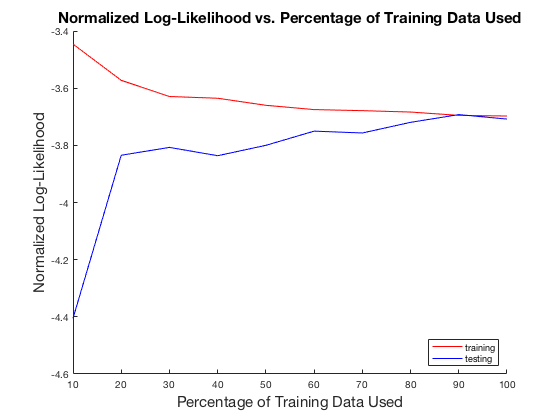
\includegraphics[scale = 0.5]{3_1_a}
    	\caption{Normalized LLH vs. Fraction of Data Used for Training}
    	\label{fig:3_1_a}
    	\end{figure}
	
        \item Mixture Models vs. Fraction of Training Data Used
        
        \begin{figure}[H]
        \centering
    	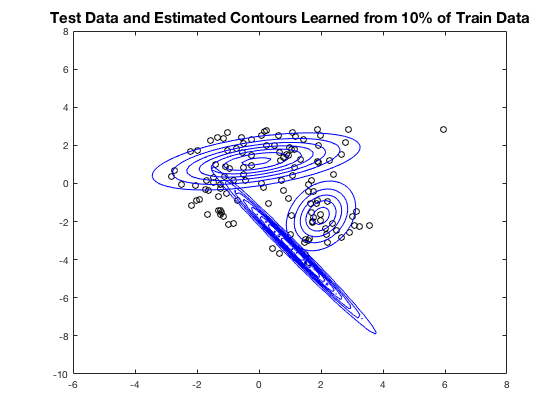
\includegraphics[scale = 0.5]{3_1_b_10}
    	\caption{10\% Data Trained On}
    	\label{fig:3_1_b_10}
    	\end{figure}
	
	\begin{figure}[H]
        \centering
    	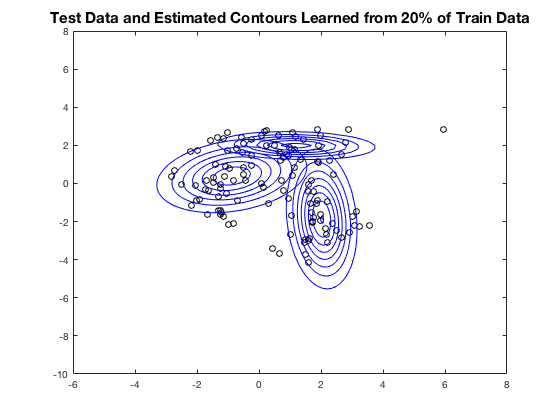
\includegraphics[scale = 0.5]{3_1_b_20}
    	\caption{20\% Data Trained On}
    	\label{fig:3_1_b_20}
    	\end{figure}
	
	\begin{figure}[H]
        \centering
    	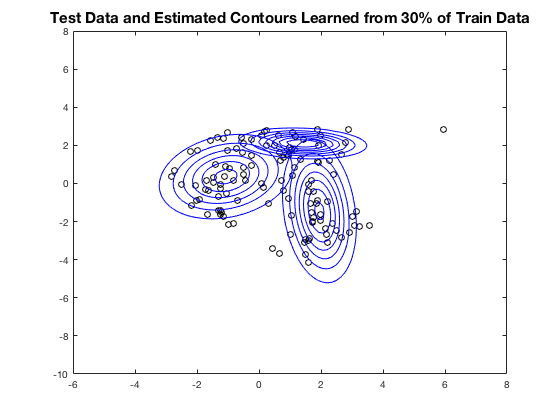
\includegraphics[scale = 0.5]{3_1_b_30}
    	\caption{30\% Data Trained On}
    	\label{fig:3_1_b_30}
    	\end{figure}
	
	\begin{figure}[H]
        \centering
    	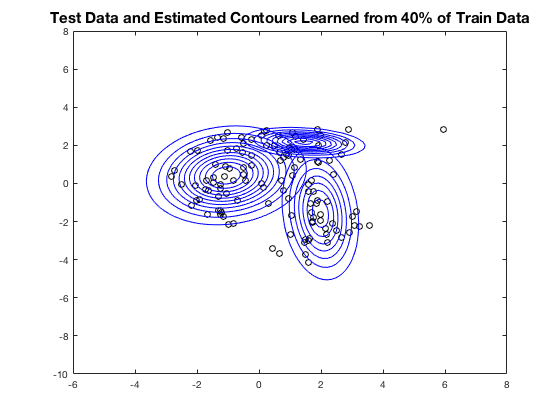
\includegraphics[scale = 0.5]{3_1_b_40}
    	\caption{40\% Data Trained On}
    	\label{fig:3_1_b_40}
    	\end{figure}
	
	\begin{figure}[H]
        \centering
    	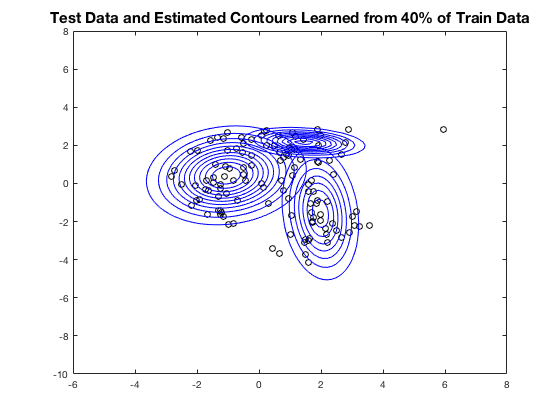
\includegraphics[scale = 0.5]{3_1_b_40}
    	\caption{40\% Data Trained On}
    	\label{fig:3_1_b_40}
    	\end{figure}
	
	\begin{figure}[H]
        \centering
    	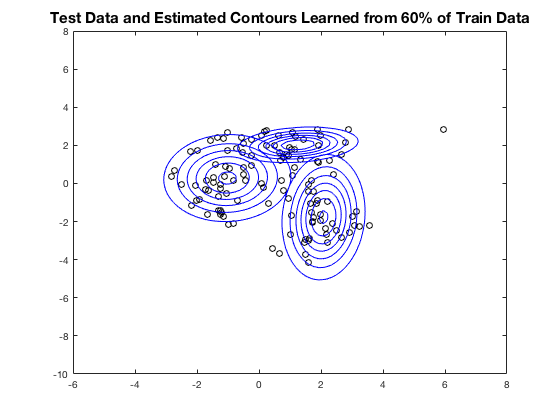
\includegraphics[scale = 0.5]{3_1_b_60}
    	\caption{60\% Data Trained On}
    	\label{fig:3_1_b_60}
    	\end{figure}
	
	\begin{figure}[H]
        \centering
    	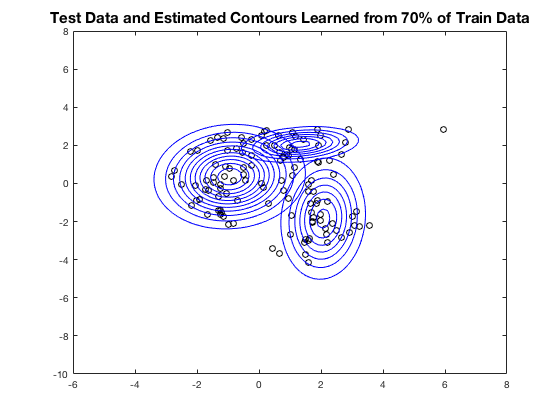
\includegraphics[scale = 0.5]{3_1_b_70}
    	\caption{70\% Data Trained On}
    	\label{fig:3_1_b_70}
    	\end{figure}
	
	\begin{figure}[H]
        \centering
    	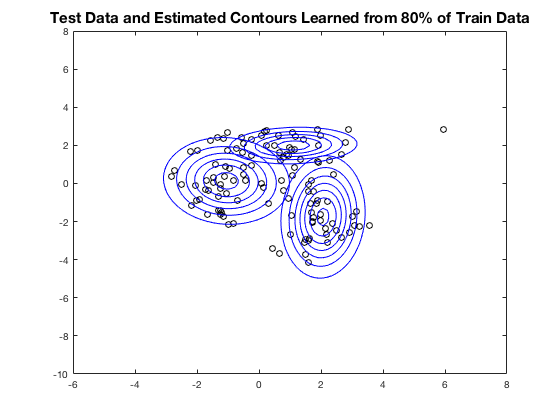
\includegraphics[scale = 0.5]{3_1_b_80}
    	\caption{80\% Data Trained On}
    	\label{fig:3_1_b_80}
    	\end{figure}
	
	\begin{figure}[H]
        \centering
    	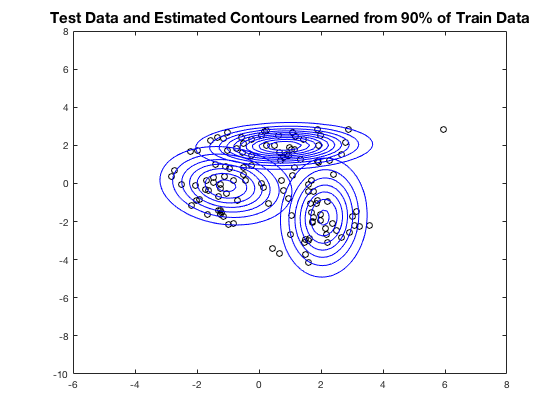
\includegraphics[scale = 0.5]{3_1_b_90}
    	\caption{90\% Data Trained On}
    	\label{fig:3_1_b_90}
    	\end{figure}
	
	\begin{figure}[H]
        \centering
    	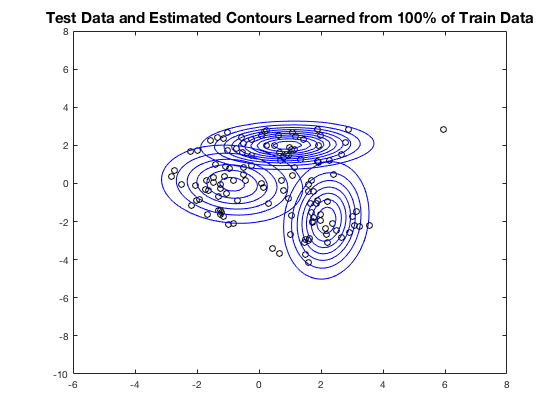
\includegraphics[scale = 0.5]{3_1_b_100}
    	\caption{100\% Data Trained On}
    	\label{fig:3_1_b_100}
    	\end{figure}
	
	When 100\% of the data is used, the parameters of the learned model are as follows:
	
	\begin{equation*}
	\bm{\mu_1} = 
	\begin{bmatrix}
	0.9146&2.0045\\
    	\end{bmatrix}~~~
  	\bm{\mu_2} = 
    	\begin{bmatrix}
    	-0.8681&-0.0383\\
	\end{bmatrix}~~~
  	\bm{\mu_3} = 
    	\begin{bmatrix}
    	2.1693&-1.9411\\
    	\end{bmatrix}
	\end{equation*}
	
	\begin{equation*}
	\Sigma_1 = 
	\begin{bmatrix}
	1.6483&0.0585\\
	0.0585&0.3369\\
    	\end{bmatrix}~~~
  	\Sigma_2 = 
    	\begin{bmatrix}
    	1.3973&-0.1459\\
    	-0.1459&1.1340\\
	\end{bmatrix}~~~
  	\Sigma_3 = 
    	\begin{bmatrix}
    	0.4589&0.1232\\
    	0.1232&2.3064\\
    	\end{bmatrix}
	\end{equation*}
	
	\begin{equation*}
	\bm{\phi} = 
	\begin{bmatrix}
	0.3118&0.3823&0.3109\\
    	\end{bmatrix}~~~
	\end{equation*}
	
	$$Normalized \;\; Train \;\; LLH = -3.6975$$
	$$Normalized \;\; Test \;\; LLH = -3.7081$$
	
	\textbf{Code for EM Algorithm}
	\color{black}
	\begin{verbatim}
function [phis, mu, sigma] = em_algorithm(X_full,K,mu)

    n = size(X_full, 1); % number of data points
    d = size(X_full, 2); % number of features

    sigma = cell(K,1); % each row corresponds to a Gaussian
    sigma(cellfun('isempty',sigma)) = {eye(d,d)};
    phis = (1/K).*ones(1,K); % each column corresponds to a Gaussian
    gammas = zeros(n,K);
    llh = compute_nllh(X_full,K,mu,sigma,phis);
    for t = 1:1000
            for j = 1:K
                numerator = phis(j) * gaussian_pdf(X_full,mu(j,:),sigma{j});
                denominator = 0;
                for m = 1:K
                    denominator = denominator + ...
                        phis(m)*gaussian_pdf(X_full,mu(m,:),sigma{m});
                end
                gammas(:,j) = numerator ./ denominator;
                N_k = sum(gammas(:,j));
                cov_new = zeros(d,d);
                mu_new = zeros(1,d);
                for i = 1:n
                    mu_new = mu_new + (gammas(i,j) .* (X_full(i,:)));
                end
                mu(j,:) = (1/N_k).*mu_new;
                for i = 1:n
                    cov_new = cov_new + ...
                        gammas(i,j).*(X_full(i,:)-mu(j,:))'*(X_full(i,:)-mu(j,:));
                end
                sigma{j} = (1/N_k).*cov_new;
                phis(j) = N_k/n;
            end
            llh_new = compute_nllh(X_full,K,mu,sigma,phis);
            if (llh_new - llh) < 10^-6
                fprintf('Broke Here at t = %d\n', t);
                break;
            else
                llh = llh_new;
            end
    end
    
end
	\end{verbatim}
	\vspace{5mm}
	\noindent\textbf{Code for 3.1}
	\color{black}
	\begin{verbatim}
	
clc; close all; clear;
normalized_llh_train = zeros(1,9);
normalized_llh_test = zeros(1,9);
K = 3;

% start in GMM_Data
for i = 1:9
    % train data
    cd TrainSubsets
    filename = sprintf('X_0.%d.mat', i);
    load(filename); % gives 'X'
    cd .. % return to GMM_Data
    cd MeanInitialization/Part_a
    filename_means = sprintf('mu_0.%d.mat', i); 
    load(filename_means); % gives 'mu'
    cd ../../ % return to GMM_Data
    [phis,mu,sigma] = em_algorithm(X,K,mu);
    normalized_llh_train(i) = compute_nllh(X,K,mu,sigma,phis);
    disp(sum(phis))
    % test data
    load('X_test.mat');
    normalized_llh_test(i) = compute_nllh(X_test,K,mu,sigma,phis);
    
    sample_plot(sigma,mu,X_test,i)
end
cd TrainSubsets
load('X_1.mat'); % gives 'X'
cd .. % return to GMM_Data
cd MeanInitialization/Part_a
load('mu_1.mat'); % gives 'mu'
cd ../../ % return to GMM_Data
[phis,mu,sigma] = em_algorithm(X,K,mu);
normalized_llh_train(10) = compute_nllh(X,K,mu,sigma,phis);
normalized_llh_test(10) = compute_nllh(X_test,K,mu,sigma,phis);

sample_plot(sigma,mu,X_test,10)

percentage = 100.*[0.1, 0.2, 0.3, 0.4, 0.5, 0.6, 0.7, 0.8, 0.9 1];
figure;
hold on
plot(percentage, normalized_llh_train, 'r');
plot(percentage, normalized_llh_test, 'b');
hold off
title('Normalized Log-Likelihood vs. Percentage of Training Data Used','FontSize',15);
xlabel('Percentage of Training Data Used','FontSize',15);
ylabel('Normalized Log-Likelihood','FontSize',15);
legend('training','testing','Location','southeast');
	\end{verbatim}

    \end{enumerate}
    
    \newpage
    \item Unknown K
    
    \begin{figure}[H]
    \centering
    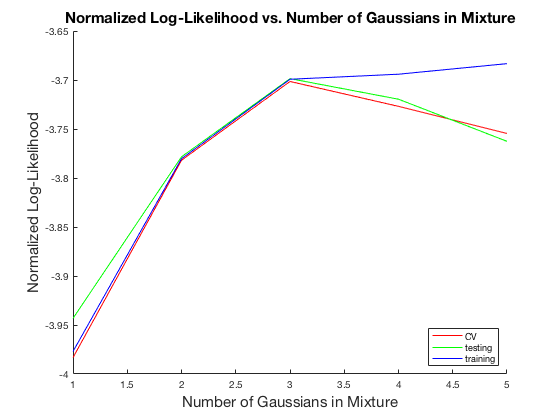
\includegraphics[scale = 0.5]{3_2}
    \caption{Normalized LLH vs. Number of Gaussians in Mixture}
    \label{fig:3_2}
    \end{figure}
    The normalized log-likelihood is the highest for $K = 3$. \\ \\
    \noindent\textbf{Code for 3.2}
    \color{black}
    \begin{verbatim}

clc; close all; clear;
K = [1, 2, 3, 4, 5];
normalized_llh_train = zeros(1,numel(K));
% normalized_llh_CV = zeros(1,numel(K));
normalized_llh_test = zeros(1,numel(K));
normalized_llh = zeros(5,5);

% start in GMM_Data
for i = 1:5 % loop over folders
    cd CrossValidation
    foldername = sprintf('Fold%d', i);
    cd(foldername)
    load('cv-train.mat'); % gives 'X_train;
    load('cv-test.mat'); % gives 'X_test;
    cd ../../ % return to GMM_Data
    for j = 1:5 % loop over Ks
        k = K(j);
        cd MeanInitialization/Part_b
        filename = sprintf('mu_k_%d.mat', j);
        load(filename); % gives 'mu'
        cd ../../ % return to GMM_Data
        [phis,mu_CV,sigma] = em_algorithm(X_train,k,mu);
        normalized_llh(i,j) = compute_nllh(X_test,k,mu_CV,sigma,phis);
        
        % train data
        load('X.mat'); % gives 'X_full'
        [phis,mu_train,sigma] = em_algorithm(X_full,k,mu);
        normalized_llh_train(j) = compute_nllh(X_full,k,mu_train,sigma,phis);
        
        % test data
        load('X_test.mat'); % gives 'X_test'
        normalized_llh_test(j) = compute_nllh(X_test,k,mu_train,sigma,phis);
    end
end
normalized_llh_CV = mean(normalized_llh,1);
figure;
hold on
plot(K, normalized_llh_CV, 'r');
plot(K, normalized_llh_test, 'g');
plot(K, normalized_llh_train, 'b');
hold off
title('Normalized Log-Likelihood vs. Number of Gaussians in Mixture','FontSize',15);
xlabel('Number of Gaussians in Mixture','FontSize',15);
ylabel('Normalized Log-Likelihood','FontSize',15);
legend('CV','testing','training','Location','southeast');
    \end{verbatim}
    
\end{enumerate}

\newpage

\section{K-means}
\begin{enumerate}
    \item The algorithm is guaranteed to converge because at each assignment step (E-Step), points are assigned to their closest centroid. There are a finite number of such assignments to be made and the number of new assignments to be made only gets smaller. This is because, once a point is assigned to a centroid, unless its an outlier, it remains in the cluster. The loss function monotonically decreases, since the distance between points in a cluster and their centroid can only get smaller as the number of iterations grows. If the distance grows, some other centroid is now closer to the point under consideration causing it to be re-assigned. Each part of the iterative update step takes the argmin of the objective function and therefore reduces it, guaranteeing convergence.
    
    \item K-means for toy dataset: \\
    Part a:
    
    \begin{figure}[H]
    \centering
    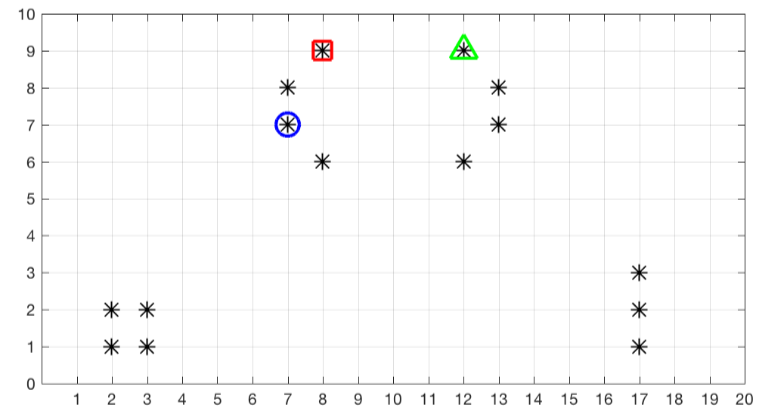
\includegraphics[scale = 0.5]{init_a}
    \caption{Centroid Initialization}
    \label{fig:init_a}
    \end{figure}
    
    \begin{figure}[H]
    \centering
    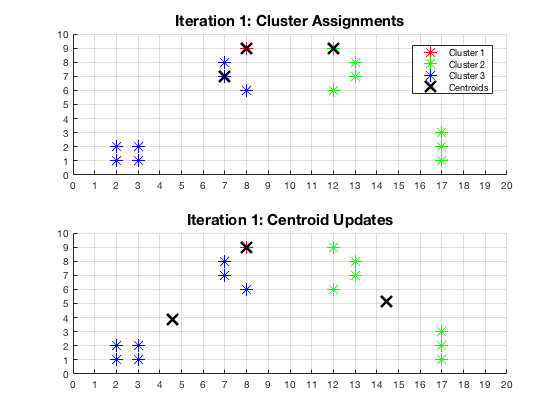
\includegraphics[scale = 0.85]{iter1_a}
    \caption{Iteration 1}
    \label{fig:iter1_a}
    \end{figure}
    
    \begin{figure}[H]
    \centering
    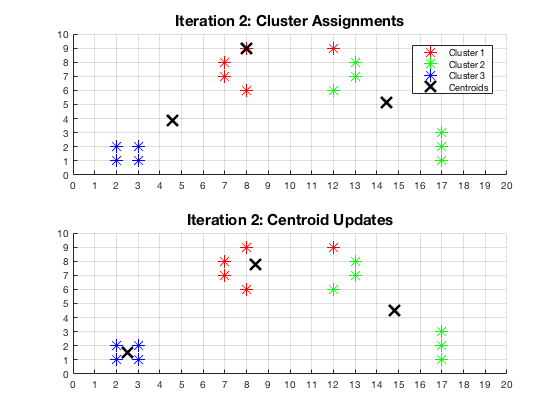
\includegraphics[scale = 0.85]{iter2_a}
    \caption{Iteration 2}
    \end{figure}
    
    \begin{figure}[H]
    \centering
    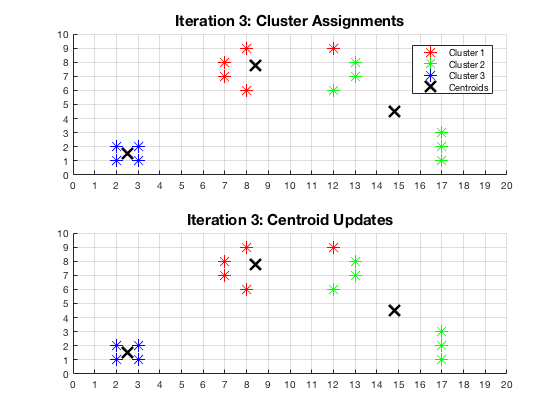
\includegraphics[scale = 0.85]{iter3_a}
    \caption{Iteration 3}
    \end{figure}
    
    \begin{figure}[H]
    \centering
    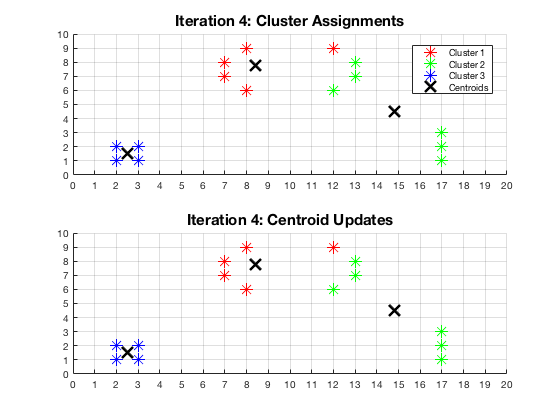
\includegraphics[scale = 0.85]{iter4_a}
    \caption{Iteration 4}
    \end{figure}
    
    \begin{figure}[H]
    \centering
    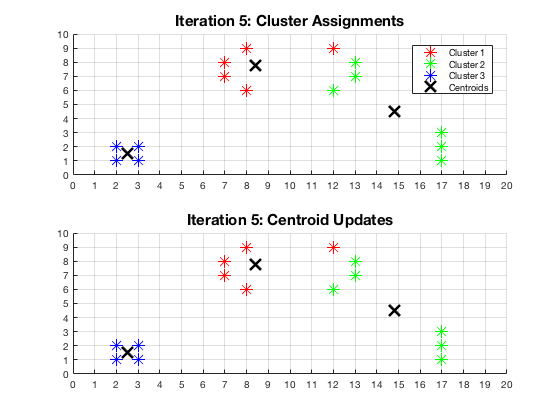
\includegraphics[scale = 0.85]{iter5_a}
    \caption{Iteration 5}
    \end{figure}
    
    \newpage
    Part b:
    
    \begin{figure}[H]
    \centering
    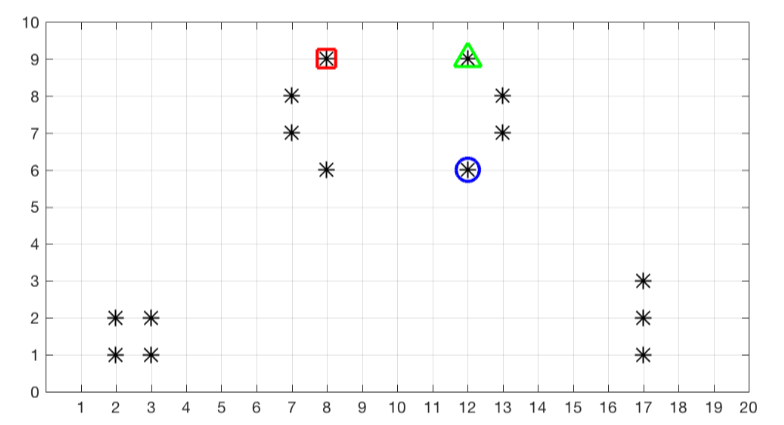
\includegraphics[scale = 0.5]{init_b}
    \caption{Centroid Initialization}
    \label{fig:init_b}
    \end{figure}
    
    \begin{figure}[H]
    \centering
    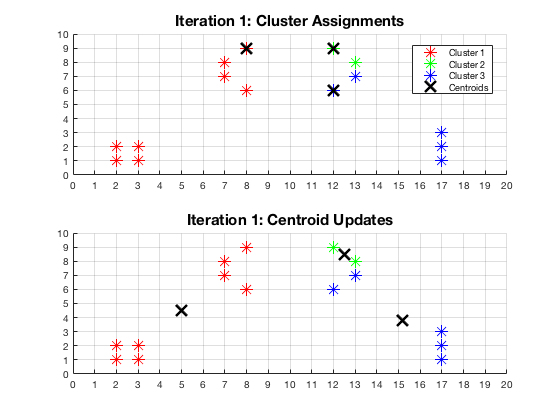
\includegraphics[scale = 0.85]{iter1_b}
    \caption{Iteration 1}
    \label{fig:iter1_b}
    \end{figure}
    
    \begin{figure}[H]
    \centering
    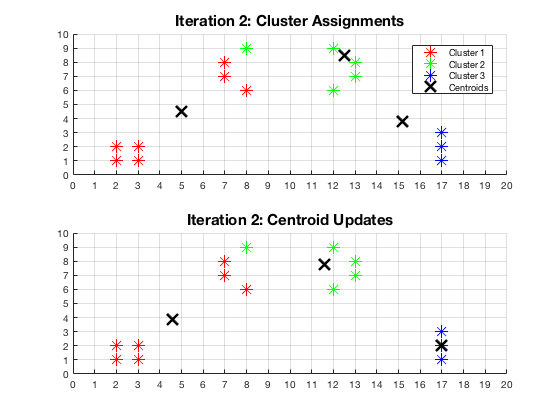
\includegraphics[scale = 0.85]{iter2_b}
    \caption{Iteration 2}
    \end{figure}
    
    \begin{figure}[H]
    \centering
    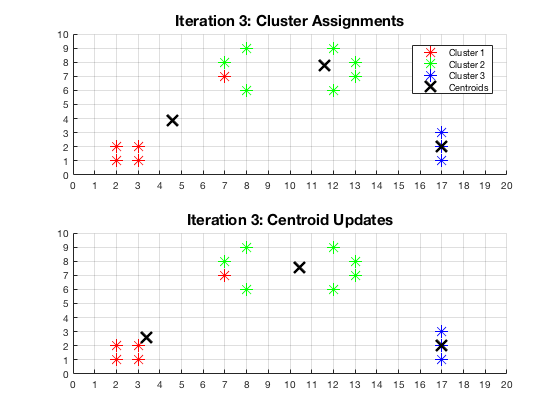
\includegraphics[scale = 0.85]{iter3_b}
    \caption{Iteration 3}
    \end{figure}
    
    \begin{figure}[H]
    \centering
    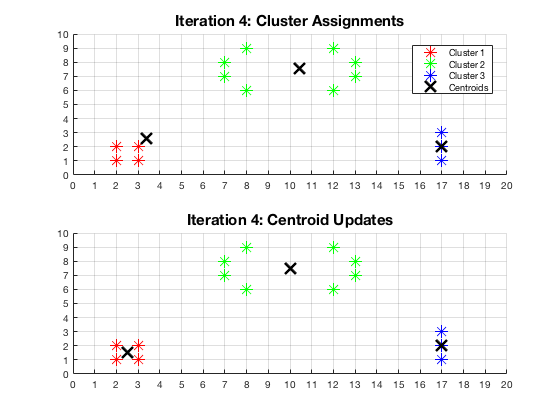
\includegraphics[scale = 0.85]{iter4_b}
    \caption{Iteration 4}
    \end{figure}
    
    \begin{figure}[H]
    \centering
    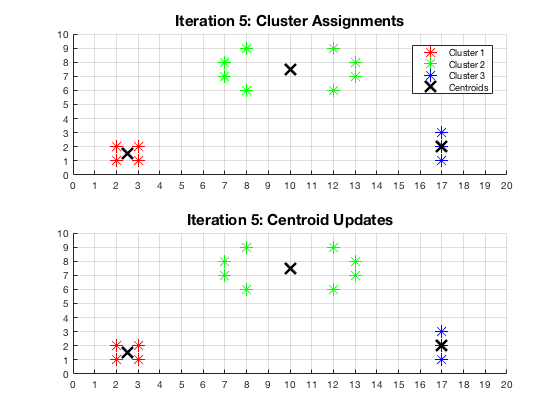
\includegraphics[scale = 0.85]{iter5_b}
    \caption{Iteration 5}
    \end{figure}
    
    \begin{figure}[H]
    \centering
    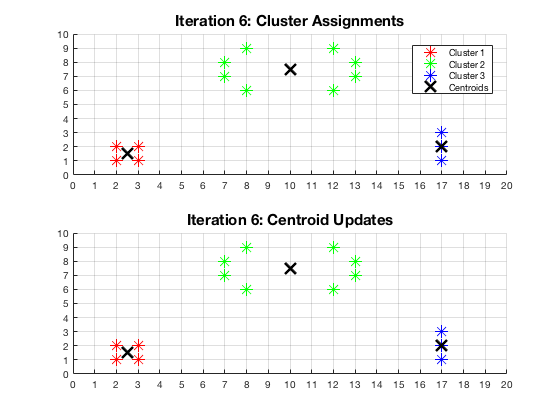
\includegraphics[scale = 0.85]{iter6_b}
    \caption{Iteration 6}
    \end{figure}
    
    \noindent\textbf{Code for K-means Iterations}
    \color{black}
    \begin{verbatim}
clc; close all; clear;
load('k_means_data.mat');

curr_centroids1 = init_centroids_1;
curr_centroids2 = init_centroids_2;

for i = 1:5
    [idx,C] = kmeans(X,3,'MaxIter',1,...
        'Start',curr_centroids1);

    figure;
    subplot(2,1,1)
    grid on;
    xlim([0 20]);
    ylim([0 10]);
    set(gca,'XTick',0:1:20);
    set(gca,'YTick',0:1:10);
    hold on
    plot(X(idx==1,1),X(idx==1,2),'r*','MarkerSize',12);
    plot(X(idx==2,1),X(idx==2,2),'g*','MarkerSize',12);
    plot(X(idx==3,1),X(idx==3,2),'b*','MarkerSize',12);
    plot(curr_centroids1(:,1),curr_centroids1(:,2),'kx',...
        'MarkerSize',15,'LineWidth',3) ;
    legend('Cluster 1','Cluster 2','Cluster 3','Centroids',...
        'Location','best');
    titletext1 = sprintf('Iteration %d: Cluster Assignments', i);
    title(titletext1,'FontSize',15);
    hold off
    curr_centroids1 = C;

    subplot(2,1,2)
    grid on;
    xlim([0 20]);
    ylim([0 10]);
    set(gca,'XTick',0:1:20);
    set(gca,'YTick',0:1:10);
    hold on
    plot(X(idx==1,1),X(idx==1,2),'r*','MarkerSize',12);
    plot(X(idx==2,1),X(idx==2,2),'g*','MarkerSize',12);
    plot(X(idx==3,1),X(idx==3,2),'b*','MarkerSize',12);
    plot(curr_centroids1(:,1),curr_centroids1(:,2),'kx',...
        'MarkerSize',15,'LineWidth',3) ;
    % legend('Cluster 1','Cluster 2','Cluster 3','Centroids',...
    %     'Location','best');
    titletext2 = sprintf('Iteration %d: Centroid Updates', i);
    title(titletext2,'FontSize',15);
    hold off
end
    
for i = 1:6
    [idx,C] = kmeans(X,3,'MaxIter',1,...
        'Start',curr_centroids2);

    figure;
    subplot(2,1,1)
    grid on;
    xlim([0 20]);
    ylim([0 10]);
    set(gca,'XTick',0:1:20);
    set(gca,'YTick',0:1:10);
    hold on
    plot(X(idx==1,1),X(idx==1,2),'r*','MarkerSize',12);
    plot(X(idx==2,1),X(idx==2,2),'g*','MarkerSize',12);
    plot(X(idx==3,1),X(idx==3,2),'b*','MarkerSize',12);
    plot(curr_centroids2(:,1),curr_centroids2(:,2),'kx',...
        'MarkerSize',15,'LineWidth',3) ;
    legend('Cluster 1','Cluster 2','Cluster 3','Centroids',...
        'Location','best');
    titletext3 = sprintf('Iteration %d: Cluster Assignments', i);
    title(titletext3,'FontSize',15);
    hold off
    curr_centroids2 = C;
    
    subplot(2,1,2)
    grid on;
    xlim([0 20]);
    ylim([0 10]);
    set(gca,'XTick',0:1:20);
    set(gca,'YTick',0:1:10);
    hold on
    plot(X(idx==1,1),X(idx==1,2),'r*','MarkerSize',12);
    plot(X(idx==2,1),X(idx==2,2),'g*','MarkerSize',12);
    plot(X(idx==3,1),X(idx==3,2),'b*','MarkerSize',12);
    plot(curr_centroids2(:,1),curr_centroids2(:,2),'kx',...
        'MarkerSize',15,'LineWidth',3) ;
    % legend('Cluster 1','Cluster 2','Cluster 3','Centroids',...
    %     'Location','best');
    titletext4 = sprintf('Iteration %d: Centroid Updates', i);
    title(titletext4,'FontSize',15);
    hold off
end
    \end{verbatim}
    
\end{enumerate}
\newpage

\section{Performance Measures for Face Detection in Images}
\begin{enumerate}
    \item Performance Metrics \\ \\
    \textbf{Group 1}
    $$TP_1 = 280$$
    $$FN_1 = 20$$
    $$FP_1 = 100$$
    $$TN_1 = 20000 - (TP_1 + FN_1 + FP_1) =19600$$
    $$TPR_1 = \frac{TP_1}{TP_1 + FN_1} = 0.9333$$
    $$TNR_1 = \frac{TN_1}{TN_1 + FP_1} = 0.9949$$
    $${Precision}_1 = \frac{TP_1}{TP_1 + FP_1} = 0.7368$$
    $$GM_1 = \sqrt{TPR_1 \times TNR_1} = 0.9636$$
    $$F1_1 = \frac{2 \times Precision_1 \times TPR_1}{Precision_1 + TPR_1} = 0.8235$$
    \\ \\ 
     \textbf{Group 2}
    $$TP_2 = 270$$
    $$FN_2 = 30$$
    $$FP_2 = 60$$
    $$TN_2 = 12500 - (TP_2 + FN_2 + FP_2) =12140$$
    $$TPR_2 = \frac{TP_2}{TP_2 + FN_2} = 0.9000$$
    $$TNR_2 = \frac{TN_2}{TN_2 + FP_2} = 0.9951$$
    $${Precision}_2 = \frac{TP_2}{TP_2 + FP_2} = 0.8182$$
    $$GM_2 = \sqrt{TPR_2 \times TNR_2} = 0.9463$$
    $$F1_2 = \frac{2 \times Precision_2 \times TPR_2}{Precision_2 + TPR_2} = 0.8571$$ 
    \\ \\
    Under the $F1$ metric, group 2's algorithm is better $(F1_2 > F1_1)$ . Under the $GM$ metric, group 1's algorithm is better $(GM_1 > GM_2)$. 
    \item The choice of metric depends on the intended application of the facial detection algorithm. The $F1$ metric takes into account the precision and the TPR. Maximizing precision places emphasis on lowering the number of false positives. The $GM$ metric takes into account the TPR and the TNR, making it closer in feel to accuracy rather than precision. If the goal is to identify not only the regions that are faces but also those that are not, the $GM$ metric is better. If the goal is to identify faces alone with less regard to the regions that are not faces, the $F1$ metric is better. 
    \end{enumerate}
\end{document}